\documentclass[a4paper,openright]{report}
% Tipo di documento. L'uso di twoside implica che i capitoli inizino sempre con la prima pagina a sinistra, eventualmente lasciando una pagina vuota nel capitolo precedente. Se questa cosa è fastidiosa, è possibile rimuoverlo. 

% Dimensione dei margini
\usepackage[a4paper,top=3cm,bottom=3cm,left=3cm,right=3cm]{geometry} 
% Dimensione del font
\usepackage[fontsize=12pt]{scrextend}
% Lingua del testo
\usepackage[italian,english]{babel}
% Lingua per la bibliografia
% \usepackage[fixlanguage]{babelbib}
% Codifica del testo
\usepackage[utf8]{inputenc} 
% Font mono (quello di default non supporta il grassetto)
\usepackage{courier}
% Encoding del testo
\usepackage[T1]{fontenc}
% Permette di generare testo fittizio. Mi è stato utile 
% per capire quale sarebbe stata l'impostazione del 
% testo nella pagina prima che scrivessi un determinato paragrafo
\usepackage{lipsum}

\usepackage[
backend=biber,
bibstyle=other/custom-numeric,
citestyle=numeric,
sorting=none,
]{biblatex}
% Sorgente della bibliografia
\addbibresource{chapters/Bibliografia.bib}

% Citazioni

% Per ruotare le immagini
\usepackage{rotating}
% Per cambiare i capitoli
\usepackage{titlesec}
% \titleformat{\chapter}[display]
  % {\normalfont\bfseries}{}{-100pt}{\huge}
\titleformat{\chapter}[hang]
  {\normalfont\bfseries\huge}{\thechapter}{1em}{\huge}
% Per mostrare nell'indice anche le subsubsection
\setcounter{tocdepth}{3}
% Per modificare l'header delle pagine 
\usepackage{fancyhdr}               

% Librerie matematiche
\usepackage{amssymb}
\usepackage{amsmath}
\usepackage{amsthm}         

% Uso delle immagini
\usepackage{graphicx}
% Uso dei colori
\usepackage[dvipsnames,svgnames,x11names]{xcolor}
% Uso dei listing per il codice
\usepackage{listings}          
% Per inserire gli hyperlinks tra i vari elementi del testo 
% \usepackage[hang, flushmargin]{footmisc}
% Diversi tipi di sottolineature
\usepackage[normalem]{ulem}

\usepackage{lstautogobble}  % Fix relative indenting
\usepackage{color}          % Code coloring
\usepackage{zi4}            % Nice font

%Aggiunti io?
\usepackage{lmodern}
\usepackage{ragged2e}
\usepackage{caption}
\usepackage[newfloat,outputdir=out]{minted}
\usepackage{float}
\usepackage[skip=5pt]{parskip}
\usepackage{setspace}
\usepackage{hyphsubst}
\usepackage{microtype}
\usepackage{hyperref}
\usepackage{footnotebackref}

% dopo minted
\usepackage{csquotes}

% subfigures
\usepackage{subcaption}

%ps to pdf
\usepackage{auto-pst-pdf}

% commento
\newcommand{\cna}[1]{{\textcolor{red}[\textcolor{red}{\bf{Avena: }}{\textcolor{red}{#1}\textcolor{red}]}}}
\newcommand{\cadm}[1]{\textcolor{cyan}[{\textcolor{cyan}{\bf{Trenitalia: }}{\textcolor{cyan}{#1}\textcolor{cyan}]}}}

% Modifica lo stile dell'header
\pagestyle{fancy}
\fancyhf{}
% \fancyhead[CE,CO]{\rightmark}
% \fancyhead[LE,RO]{\textbf{\thepage}}
\fancyhead[L]{\rightmark}
\fancyhead[R]{\textbf{\thepage}}
\fancyfoot{}
\setlength{\headheight}{17pt}

% Rimuove il numero di pagina all'inizio dei capitoli
\fancypagestyle{plain}{
  \fancyfoot{}
  \fancyhead{}
  \renewcommand{\headrulewidth}{0pt}
}

% Togliendo il commento al comando che segue, si inseriscono nella bibliografia anche le fonti presenti in Bibliography.bib ma non citati direttamente con il comando \cite

% Modifica dello stile dei riferimenti, con il testo in cyano
\definecolor{DarkGreen}{RGB}{20,80,40}
\definecolor{Unipi}{RGB}{00,85,143} 
\definecolor{term_bg_color}{RGB}{240,241,240} 
\hypersetup{
    colorlinks,
    linkcolor=Unipi,
    citecolor=Unipi,
    urlcolor=Unipi
}


\DeclareCiteCommand{\supercite}[\mkbibsuperscript]
  {\iffieldundef{prenote}
     {}
     {\BibliographyWarning{Ignoring prenote argument}}%
   \iffieldundef{postnote}
     {}
     {\BibliographyWarning{Ignoring postnote argument}}}
  {\usebibmacro{citeindex}%
   \bibopenbracket\usebibmacro{cite}\bibclosebracket}
  {\supercitedelim}
  {}


% Aggiunti definizioni, teoremi, linea e listing
\newtheorem{definition}{Definizione}[section]
\newtheorem{theorem}{Teorema}[section]
\providecommand*\definitionautorefname{Definizione}
\providecommand*\theoremautorefname{Teorema}
\providecommand*{\listingautorefname}{Listing}
\providecommand*\lstnumberautorefname{Linea}

\raggedbottom

\usepackage{tcolorbox}
\usepackage{xpatch}


% -----------------------------------------------------------------

\begin{document}

\setlength{\fboxsep}{0pt}
\selectlanguage{english}

% \hyphenpenalty=10000
% \exhyphenpenalty=10000

% \loadspellchecklist[it][wordlist.txt]
% \setupspellchecking[state=start]

\setminted{
    linenos=true,
    numbersep=5pt,
    bgcolor=term_bg_color,
    frame=single,
    framesep=5pt,
    tabsize=2,
    breaklines=true,
    baselinestretch=0.9
}

\setlength{\abovecaptionskip}{-2pt} 
\setlength{\belowcaptionskip}{8pt} 

\newenvironment{code}
    {\captionsetup{type=listing}}
    {\par\noindent\ignorespacesafterend}

\SetupFloatingEnvironment{listing}{name=Listing, listname=List of Listings}

\usemintedstyle{sas}
% \usemintedstyle{unipi}
% \usemintedstyle{xcode}
% \usemintedstyle[output]{rrt}

% Interlinea
\setstretch{1.1}

\begin{titlepage}
\begin{figure}[!htb]

\begin{center}
{
    
\includegraphics[keepaspectratio=true,scale=0.5]{images/Frontespizio/cherubinFrontespizio.eps}
}
\end{center}

\end{figure}

\begin{center}
    \LARGE{UNIVERSITÀ DI PISA}
\end{center}

\vspace{15mm}
\begin{center}
    {\LARGE{\bf CORDIC: Cartesian to  \\ \vspace{3mm} Polar Coordinate Transformation }}
\end{center}
\vspace{30mm}

\vfill
\hrulefill
\\\centering{\large{ANNO ACCADEMICO 2024/2025}}

\end{titlepage}
\stepcounter{page}

\tableofcontents


\chapter{Introduction}

\section{Specification}

\section{Circuit Applications}
\chapter{Architecture}

\chapter{VHDL code}


\section{CORDIC}
The following code shows the implementation of the CORDIC in vectoring mode for cartesian to polar conversion. This implementation supports the fix step for accepting inputs in all 4 quadrants, and also normalizes \( \rho \).

\begin{code}
    \vhdlCode{../vhdl/src/CORDIC.vhd}
    \captionof{listing}{\texttt{CORDIC.vhd}}
    \label{code:vhdl}
\end{code}


\section{Atan LUT}
The values of the LUT table were calculated using the formula:
\[
    \text{LUT}_i = \left\lfloor \text{atan}(2^{-i} )* 2^{21} \right\rfloor
\]
\begin{code}
    \vhdlCode{../vhdl/src/ATAN_LUT.vhd}
    \captionof{listing}{\texttt{ATAN\_LUT.vhd}}
    \label{code:lut}
\end{code}

\chapter{Verification and testing}

\section{Testbench}



\begin{code}
    \inputminted{vhdl}{listings/04/CORDIC_tb.vhd}
    \captionof{listing}{\texttt{CORDIC\_tb.vhd}}
    \label{code:testbench}
\end{code}

\chapter{Vivado results}
After completing the verification phase, the circuit design was synthesized and implemented using the Vivado Tool, specifically targeting the Zybo Zynq-7010 development board.

\section{Vivado Design flow}
For the implementation of the CORDIC algorithm in vectoring mode for Cartesian-to-Polar conversion, the Vivado design flow was employed using Xilinx/AMD Vivado software. This process involved RTL Elaboration, Synthesis, and Implementation on the target FPGA, along with the application of design constraints and the extraction of power and timing reports. To ensure accurate and reliable timing analysis, all combinational logic paths were structured to follow a Register-Logic-Register configuration.

\section{RTL}
Vivado produced a logic network made of:

% todo cambiare numeri
\begin{enumerate}
    \item 144 cells (e.g. multiplexers, DFFs, adders)
    \item 68 I/O ports ($16_{x} + 16_{y} + 16_{\rho} + 16_{\theta} + 1_{clk} + 1_{rst} + 1_{start} + 1_{valid}$)
    \item 802 nets (for connecting all the components)
\end{enumerate}

The RTL Analysis generated the Elaborated Design shown in Figure \ref{fig:schematic}, consistent with the expected structure of the system.

\begin{figure}[H]
    \centering
    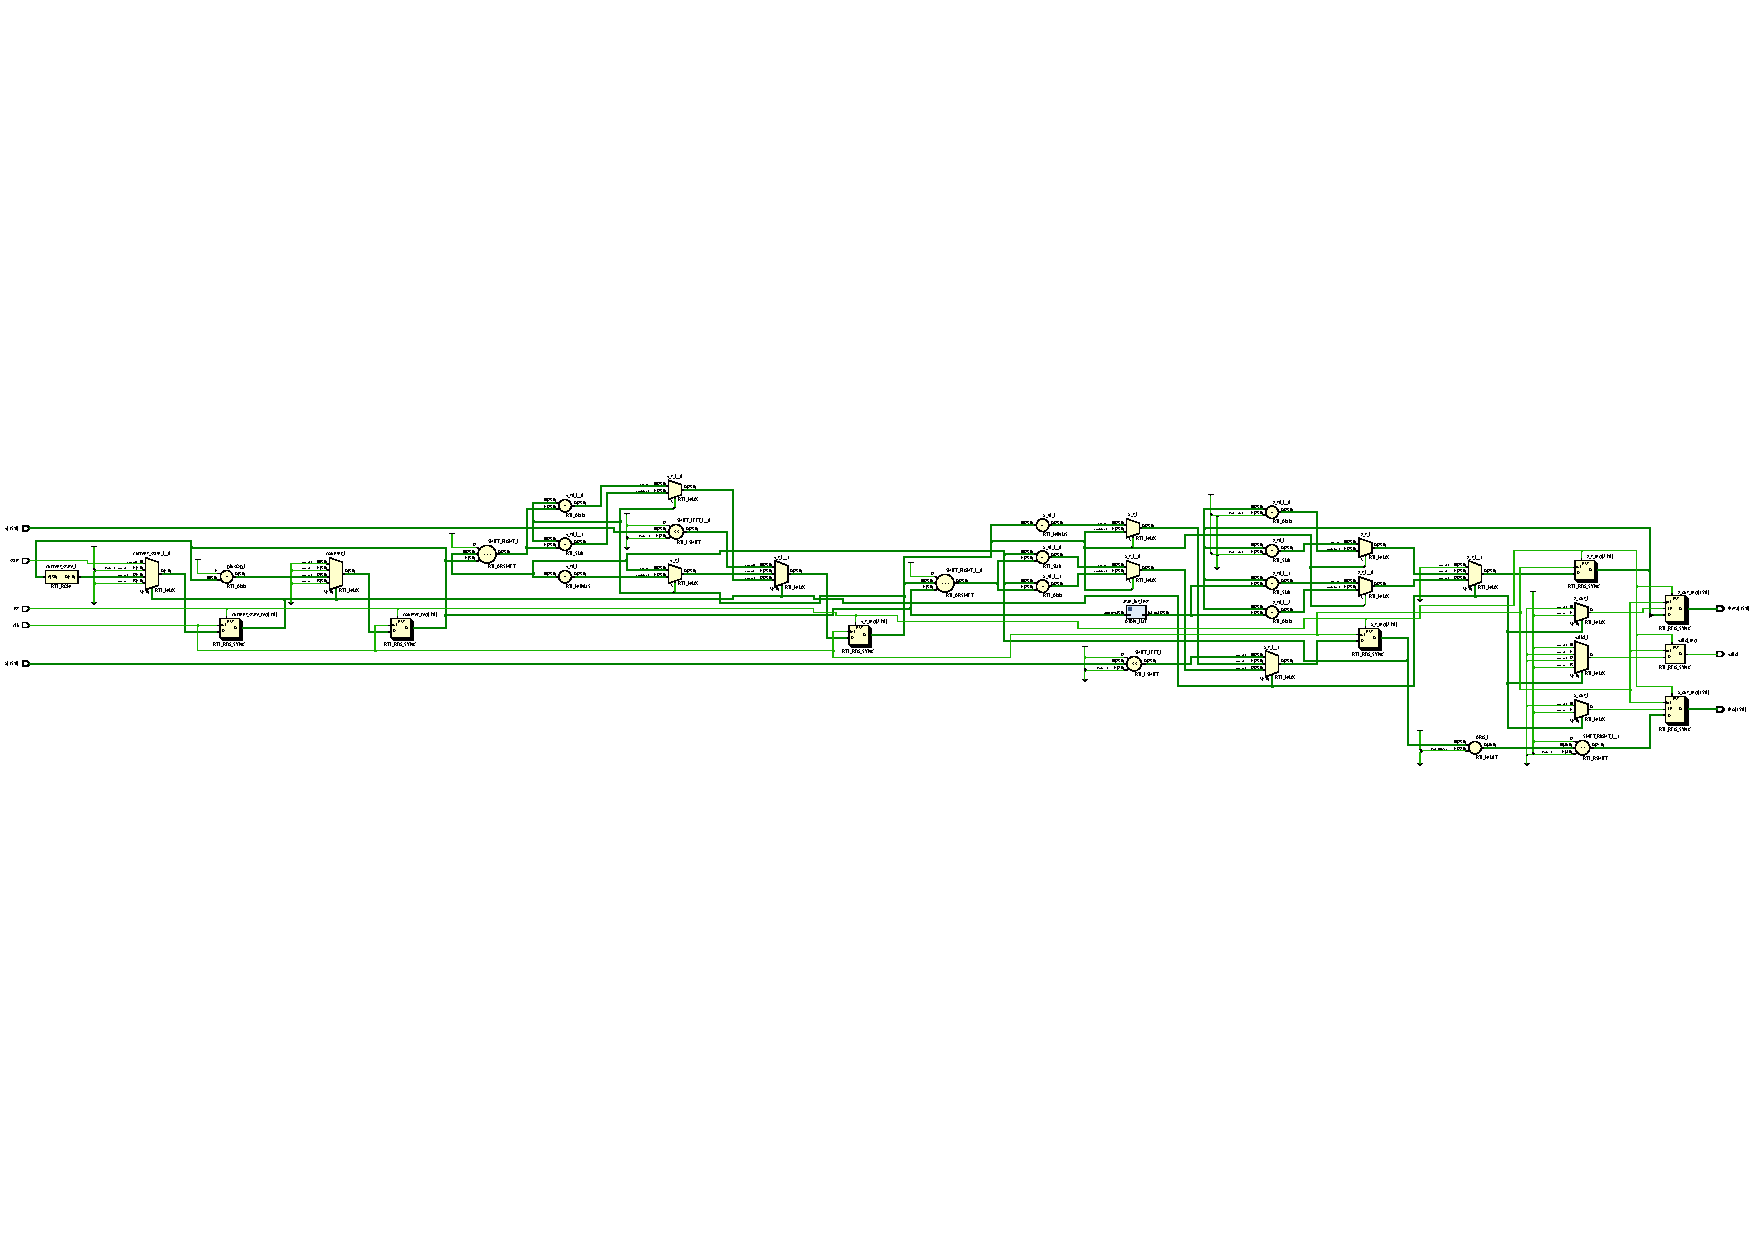
\includegraphics[width=\textwidth, trim=0 200 0 200, clip]{./images/Vivado/rtl.pdf}
    \caption{Elaborated RTL design.}
    \label{fig:schematic}
\end{figure}

\section{Synthesis timing report}
\begin{figure}[H]
    \centering
    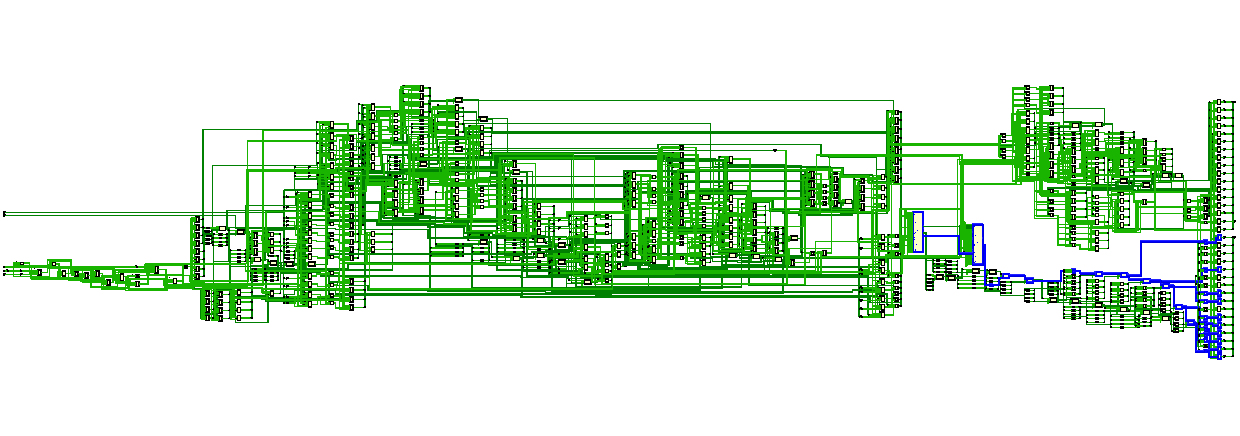
\includegraphics[width=\textwidth, trim=0 160 0 160, clip]{./images/Vivado/setup_synthesis.pdf}
    \caption{Figure showing the elaborated RTL design with the main critical paths for set-up-time-violation found in synthesis step highlighted in blue.}
    \label{fig:setup_synthesis}
\end{figure}

\begin{table}[H]
    \centering
    \small
    \captionsetup{skip=10pt} 
    \begin{tabular}{lrrrrrrr}
        \hline
        Name &  Slack &  Levels &  Routes & From      & To                 & Total Delay    \\
        \hline
        Path 1 &  12.78 &      10 &       6 & y\_t\_reg[14]/C  & ARG/A[23]       &         6.77   \\
        Path 2 &  12.78 &      10 &       6 & y\_t\_reg[14]/C  & ARG\_\_0/A[23]  &         6.77   \\
        Path 3 &  12.90 &       9 &       6 & y\_t\_reg[14]/C  & ARG/A[19]       &         6.66   \\
        Path 4 &  12.90 &       9 &       6 & y\_t\_reg[14]/C  & ARG\_\_0/A[19]  &         6.66   \\
        Path 5 &  13.02 &       8 &       6 & y\_t\_reg[14]/C  & ARG/A[15]       &         6.54   \\
        Path 6 &  13.02 &       8 &       6 & y\_t\_reg[14]/C  & ARG\_\_0/A[15]  &         6.54   \\
        Path 7 &  13.03 &      10 &       6 & y\_t\_reg[14]/C  & ARG/A[22]       &         6.53   \\
        Path 8 &  13.03 &      10 &       6 & y\_t\_reg[14]/C  & ARG\_\_0/A[22]  &         6.53   \\
        Path 9 &  13.08 &      10 &       6 & y\_t\_reg[14]/C  & ARG/A[21]       &         6.47   \\
        Path 10 &  13.08 &      10 &       6 & y\_t\_reg[14]/C  & ARG\_\_0/A[21]  &         6.47   \\
        \hline
    \end{tabular}
    \caption{Table showing data of the main critical paths found in synthesis step}
    \label{tab:setup_synthesis}
\end{table}
    
\begin{figure}[H]
    \centering
    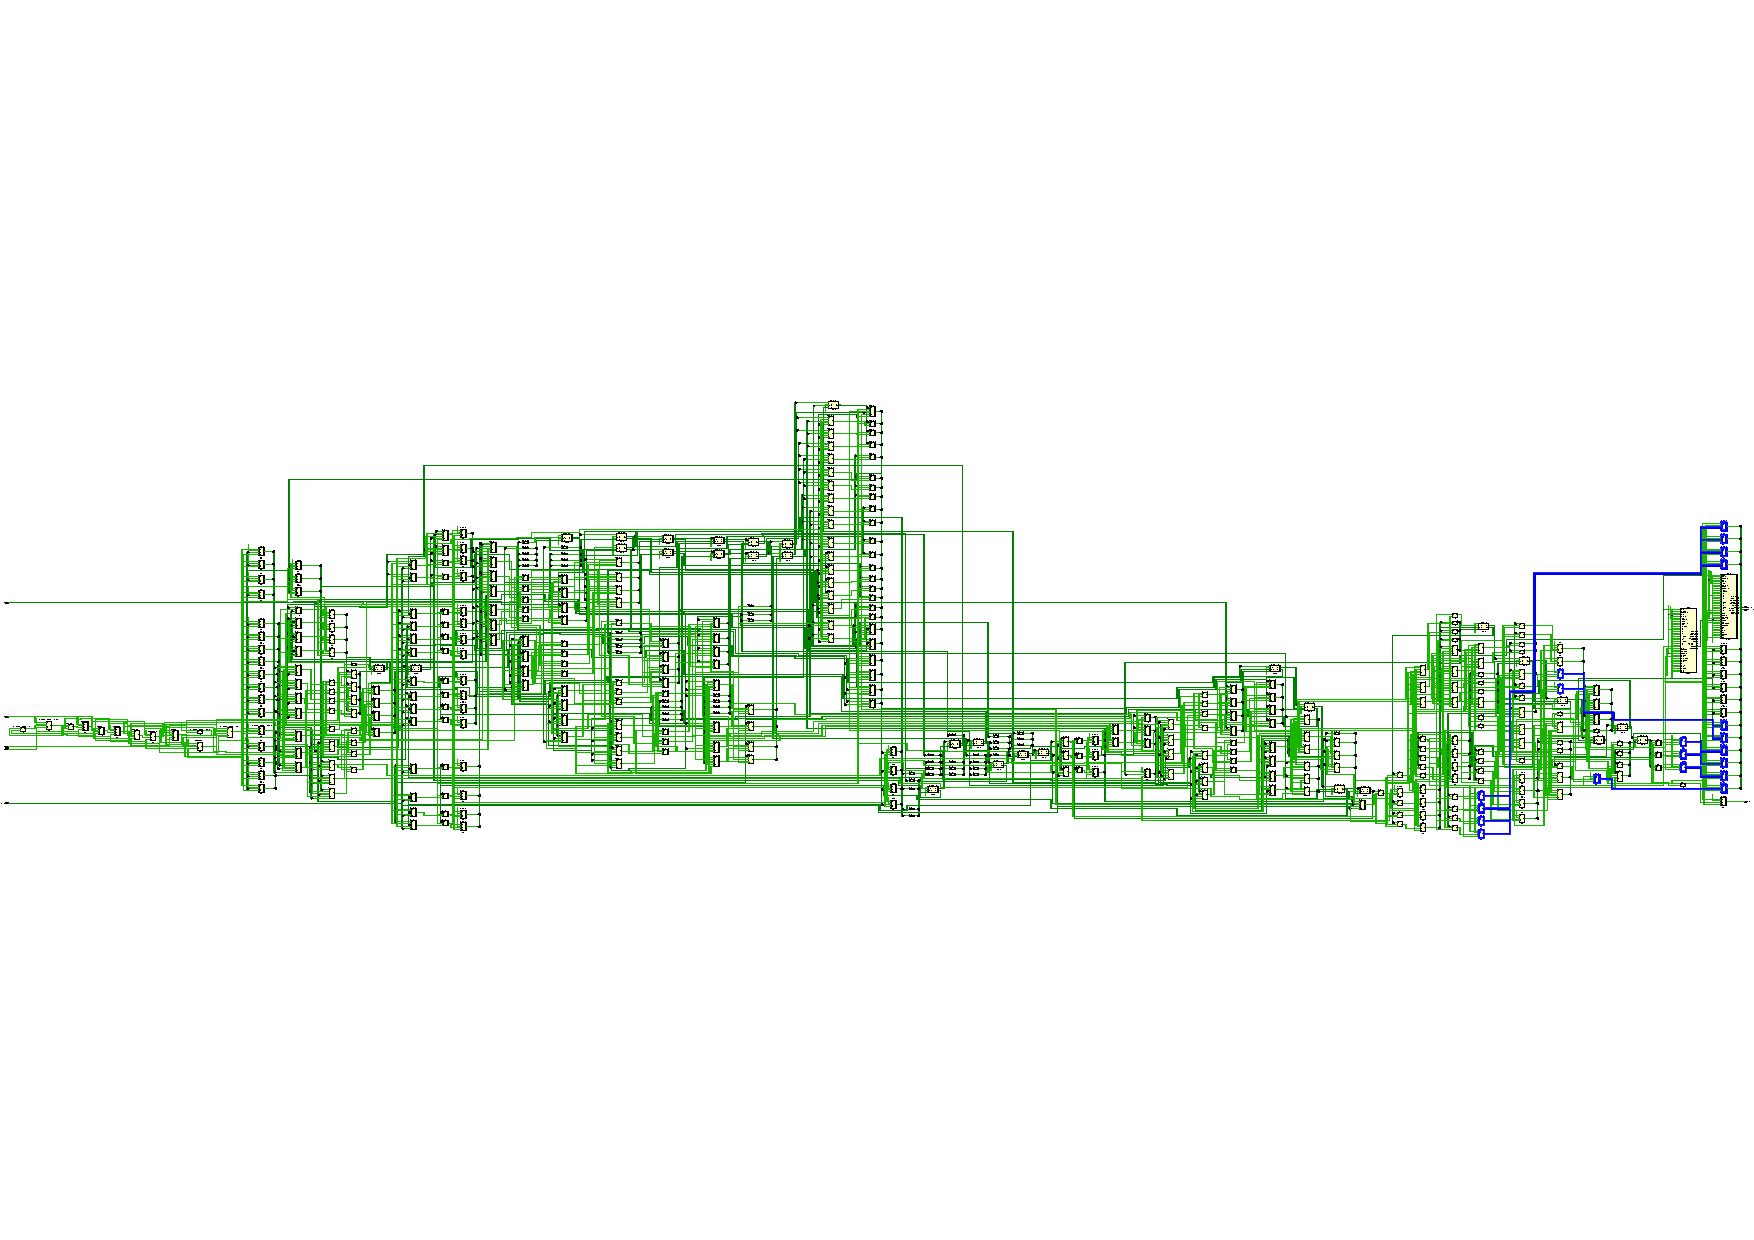
\includegraphics[width=\textwidth, trim=0 160 0 160, clip]{./images/Vivado/hold_synthesis.pdf}
    \caption{Figure showing the elaborated RTL design with the main critical paths for hold-time-violation found in synthesis step highlighted in blue.}
    \label{fig:hold_synthesis}
\end{figure}  

\begin{table}[H]
    \centering
    \small
    \captionsetup{skip=10pt} 
    \begin{tabular}{lrrrrrr}
        \hline
        Name    & Slack & Levels & Routes  & From           & To               & Total Delay \\
        \hline
        Path 11 &  0.28 &      0 &       1 & z\_t\_reg[23]/C & z\_out\_reg[15]/D & 0.30       \\
        Path 12 &  0.28 &      0 &       1 & z\_t\_reg[8]/C  & z\_out\_reg[0]/D  & 0.31       \\
        Path 13 &  0.28 &      0 &       1 & z\_t\_reg[18]/C & z\_out\_reg[10]/D & 0.31       \\
        Path 14 &  0.28 &      0 &       1 & z\_t\_reg[19]/C & z\_out\_reg[11]/D & 0.31       \\
        Path 15 &  0.28 &      0 &       1 & z\_t\_reg[20]/C & z\_out\_reg[12]/D & 0.31       \\
        Path 16 &  0.28 &      0 &       1 & z\_t\_reg[21]/C & z\_out\_reg[13]/D & 0.31       \\
        Path 17 &  0.28 &      0 &       1 & z\_t\_reg[22]/C & z\_out\_reg[14]/D & 0.31       \\
        Path 18 &  0.28 &      0 &       1 & z\_t\_reg[9]/C  & z\_out\_reg[1]/D  & 0.31       \\
        Path 19 &  0.28 &      0 &       1 & z\_t\_reg[10]/C & z\_out\_reg[2]/D  & 0.31       \\
        Path 20 &  0.28 &      0 &       1 & z\_t\_reg[11]/C & z\_out\_reg[3]/D  & 0.31       \\
        \hline
    \end{tabular}
    \caption{Table showing the characteristics regarding critical paths for hold-time-violation found in synthesis step.}
    \label{tab:hold_synthesis}
\end{table}



\section{Implementation timing report}

\begin{figure}[H]
    \centering
    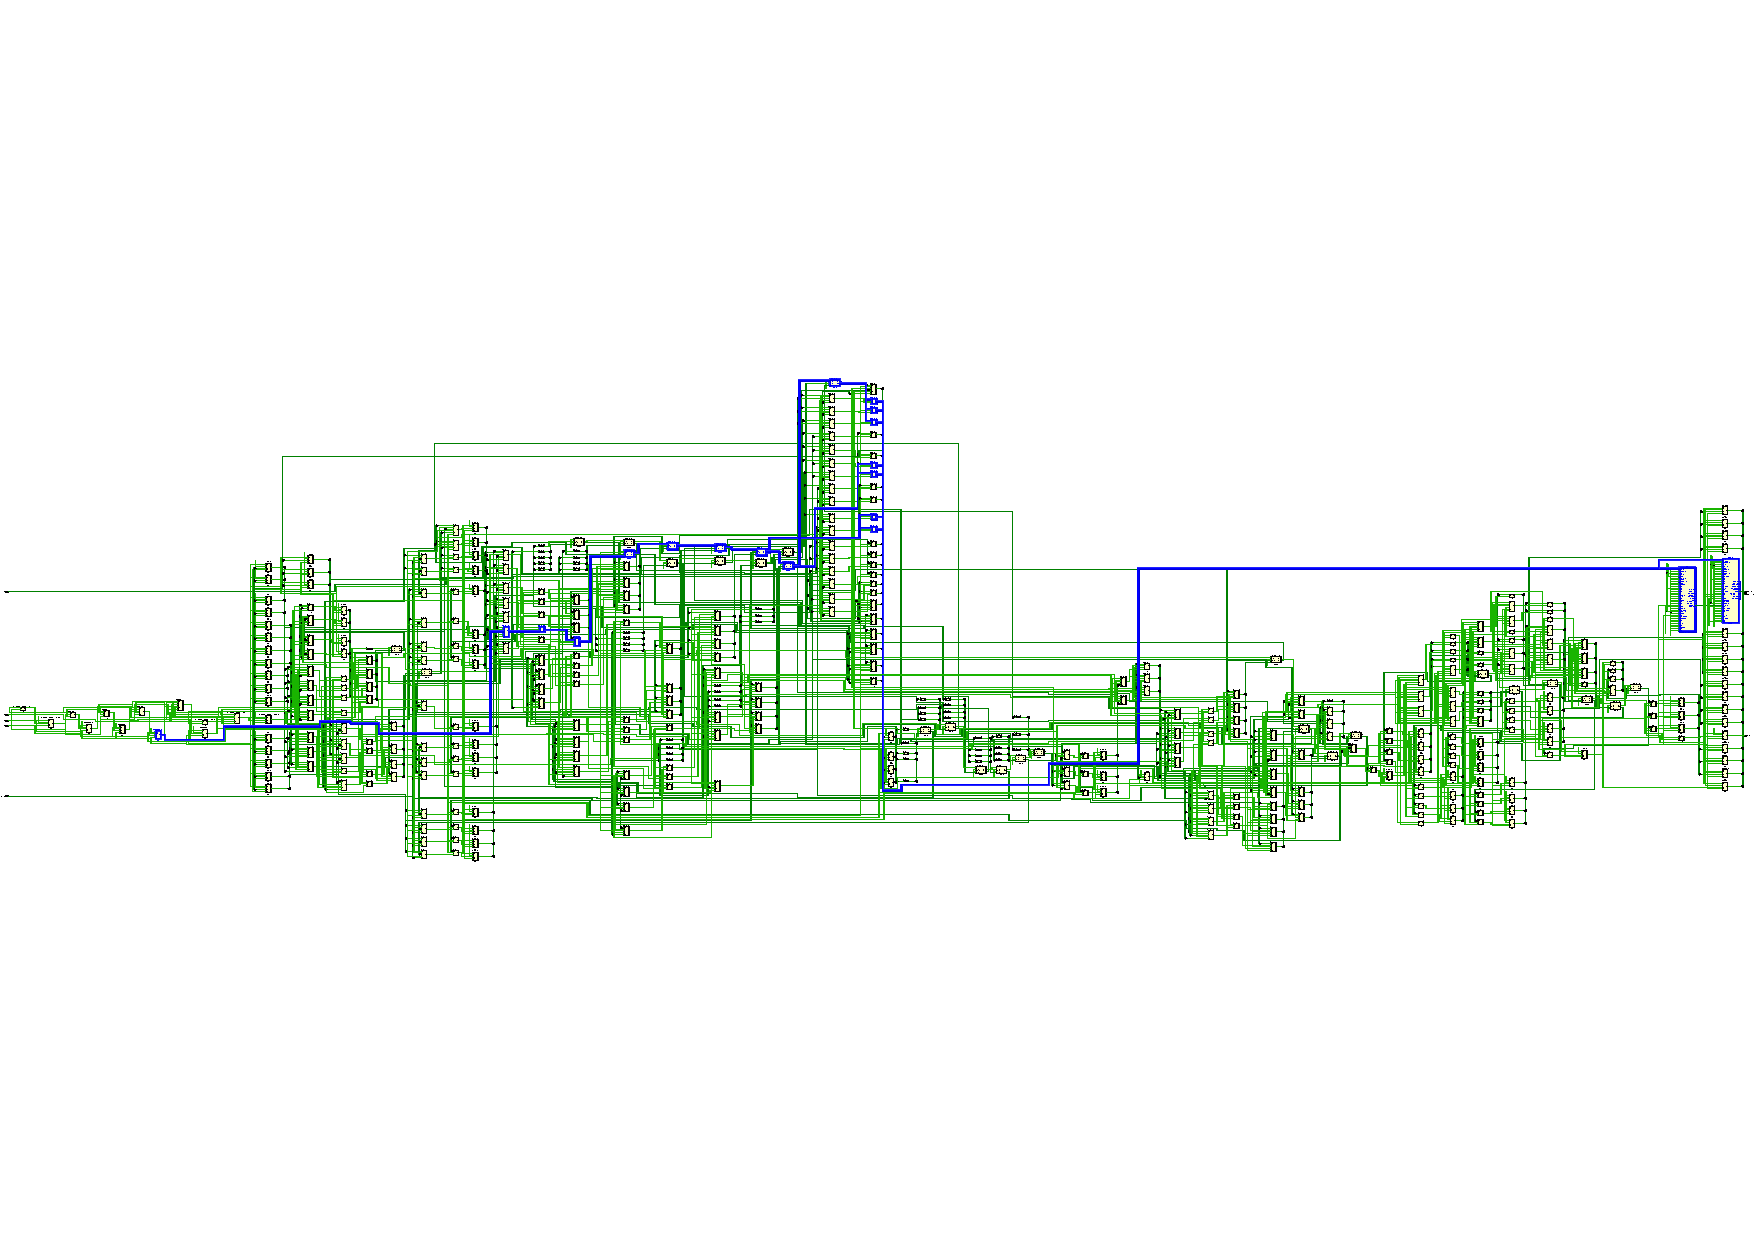
\includegraphics[width=\textwidth, trim=0 160 0 160, clip]{./images/Vivado/setup_implementation.pdf}
    \caption{Figure showing the elaborated RTL design with the main critical paths for set-up-time-violation found during implementation step highlighted in blue.}
    \label{fig:setup_implementation}
\end{figure}

\begin{table}[H]
    \centering
    \small
    \captionsetup{skip=10pt} 
    \begin{tabular}{lrrrrrr}
        \hline
        Name    & Slack & Levels & Routes  & From           & To               & Total Delay \\
        \hline
        Path 1  & 10.19 &      10 &       6 & counter\_reg[2]/C & ARG/A[20]        & 9.16       \\
        Path 2  & 10.38 &      10 &       6 & counter\_reg[2]/C & ARG\_\_0/A[20]   & 8.97       \\
        Path 3  & 10.43 &      10 &       6 & counter\_reg[2]/C & ARG\_\_0/A[21]   & 9.13       \\
        Path 4  & 10.43 &      10 &       6 & counter\_reg[2]/C & ARG/A[22]        & 8.92       \\
        Path 5  & 10.57 &       8 &       6 & counter\_reg[2]/C & ARG\_\_0/A[12]   & 8.78       \\
        Path 6  & 10.59 &       9 &       6 & counter\_reg[2]/C & ARG\_\_0/A[17]   & 8.97       \\
        Path 7  & 10.60 &       9 &       6 & counter\_reg[2]/C & ARG/A[16]        & 8.75       \\
        Path 8  & 10.61 &       8 &       6 & counter\_reg[2]/C & ARG\_\_0/A[13]   & 8.94       \\
        Path 9  & 10.61 &      10 &       6 & counter\_reg[2]/C & ARG/A[21]        & 8.94       \\
        Path 10 & 10.62 &      10 &       6 & counter\_reg[2]/C & ARG\_\_0/A[22]   & 8.73       \\
        \hline
    \end{tabular}
    \caption{Table showing the main critical paths for the setup-time-violation during the implementation step.}
    \label{tab:setup_implementation}
\end{table}


\begin{figure}[H]
    \centering
    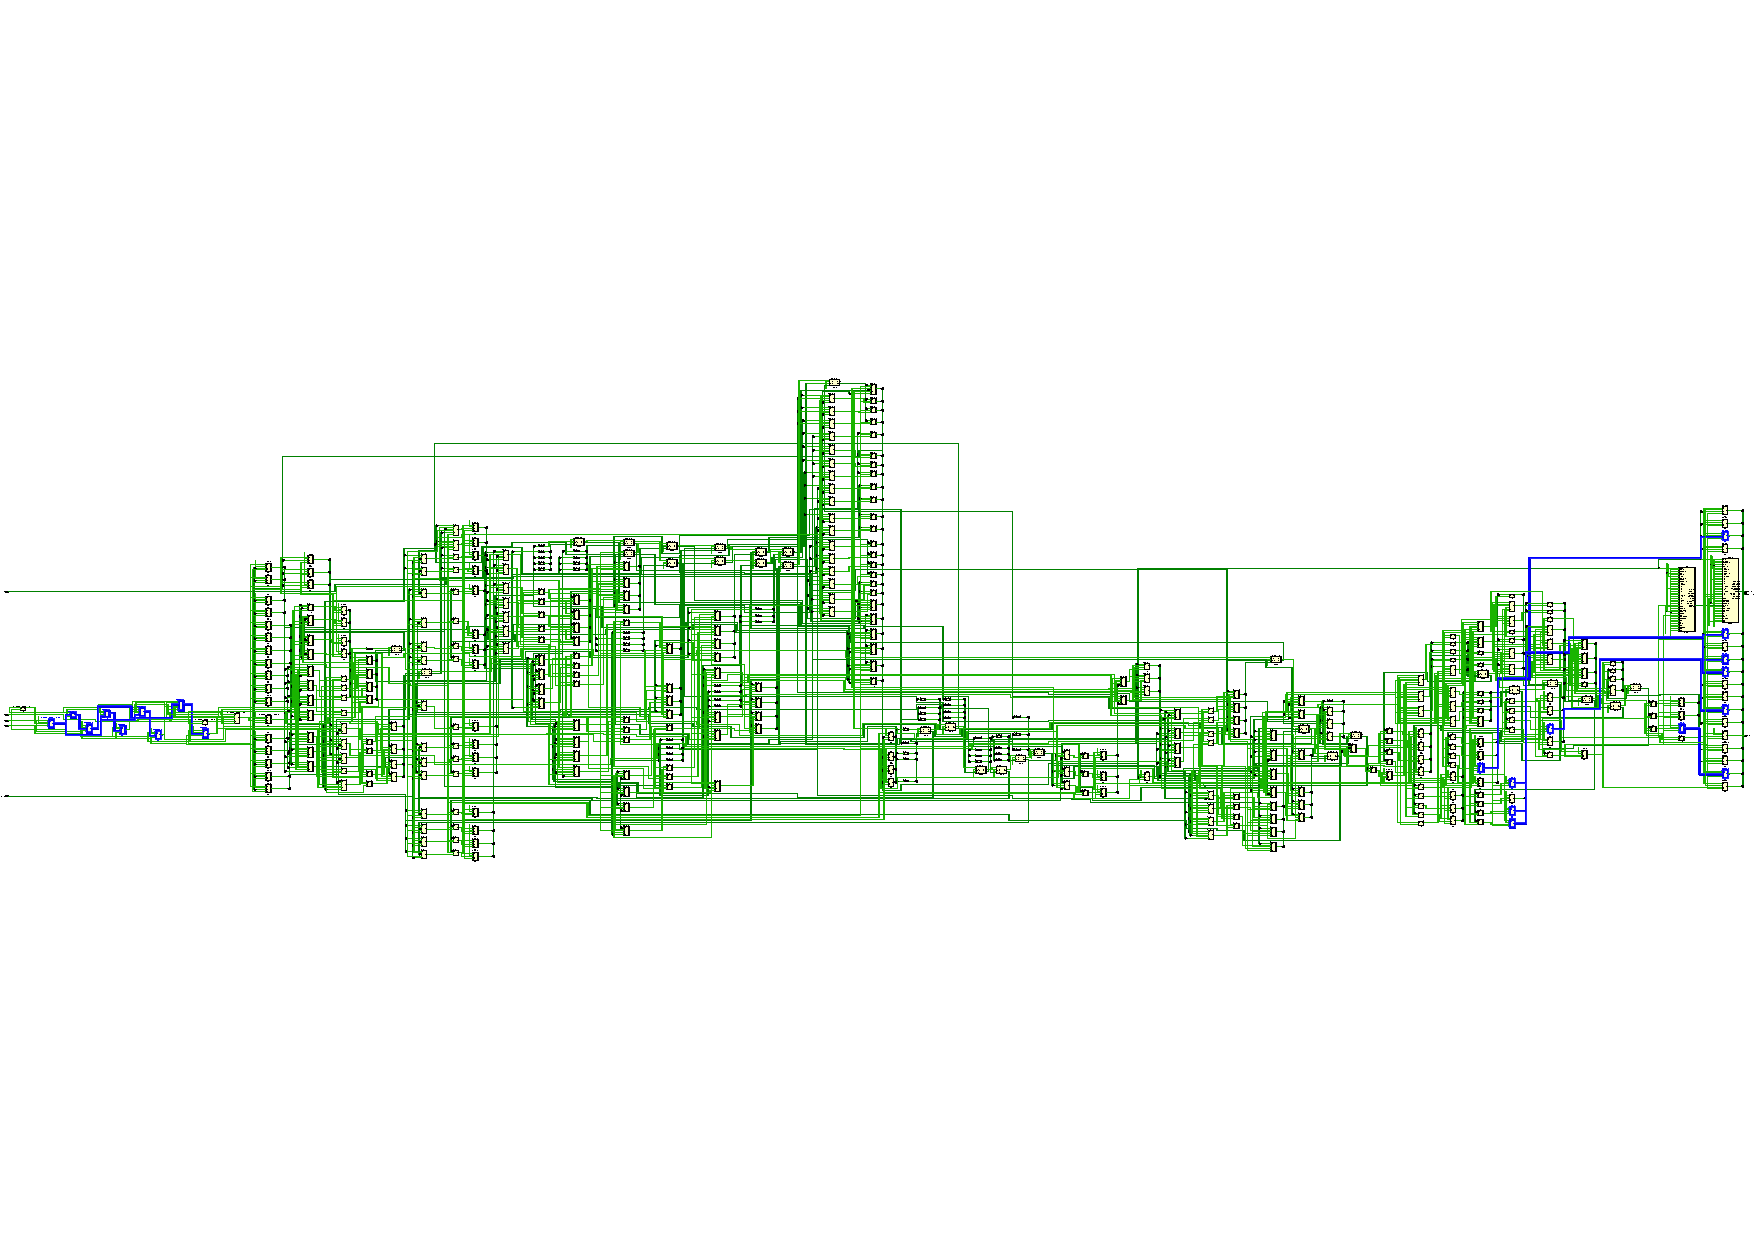
\includegraphics[width=\textwidth, trim=0 160 0 160, clip]{./images/Vivado/hold_implementation.pdf}
    \caption{Figure showing the elaborated RTL design with the main critical paths for hold-time-violation found during implementation step highlighted in blue.}
    \label{fig:hold_implementation}
\end{figure}

\begin{table}[H]
    \centering
    \small
    \captionsetup{skip=10pt} 
    \begin{tabular}{lrrrrrr}
        \hline
        Name    & Slack & Levels   & From                              & To                    & Total Delay \\
        \hline
        Path 11 &  0.17 &       1 &  current\_state\_reg[1]/C & counter\_reg[2]/D     & 0.33       \\
        Path 12 &  0.18 &       1 &  current\_state\_reg[1]/C & counter\_reg[0]/D     & 0.32       \\
        Path 13 &  0.18 &       1 &  current\_state\_reg[1]/C & counter\_reg[1]/D     & 0.32       \\
        Path 14 &  0.19 &       0 &  z\_t\_reg[22]/C                  & z\_out\_reg[14]/D     & 0.29       \\
        Path 15 &  0.22 &       0 &  z\_t\_reg[12]/C                  & z\_out\_reg[4]/D      & 0.29       \\
        Path 16 &  0.22 &       0 &  z\_t\_reg[14]/C                  & z\_out\_reg[6]/D      & 0.30       \\
        Path 17 &  0.23 &       0 &  z\_t\_reg[15]/C                  & z\_out\_reg[7]/D      & 0.26       \\
        Path 18 &  0.23 &       0 &  z\_t\_reg[10]/C                  & z\_out\_reg[2]/D      & 0.33       \\
        Path 19 &  0.24 &       1 &  counter\_reg[0]/C                & counter\_reg[3]/D     & 0.38       \\
        Path 20 &  0.24 &       0 &  z\_t\_reg[18]/C                  & z\_out\_reg[10]/D     & 0.32       \\
        \hline
    \end{tabular}
    \caption{Table showing the main critical paths for hold-time-violation found in the implementation step.}
    \label{tab:hold_implementation}
\end{table}

\section{Utilization Report}
\begin{table}[H]
    \centering
    \small
    \captionsetup{skip=10pt} 
    \begin{tabular}{lrr}
        \hline
        Resource               & Utilization (\%) & Description \\
        \hline
        Slice LUTs             & 1.59\%           & Look-Up Tables used as logic \\
        Slice Registers        & 0.27\%           & Registers used in the design \\
        Slice                  & 1.93\%           & Total slices utilized \\
        LUT as Logic           & 1.59\%           & LUTs specifically used as logic \\
        DSPs                   & 2.50\%           & Digital Signal Processing blocks \\
        Bonded IOB             & 0.00\%           & Bonded Input/Output Blocks \\
        BUFGCTRL               & 0.00\%           & Global Clock Buffers \\
        \hline
    \end{tabular}
    \caption{Resource utilization for the CORDIC design (only non-zero values shown)}
    \label{tab:cordic_resource_utilization}
\end{table}


\section{Power Report}
\begin{figure}[H]
    \centering
    \captionsetup{skip=10pt} 
    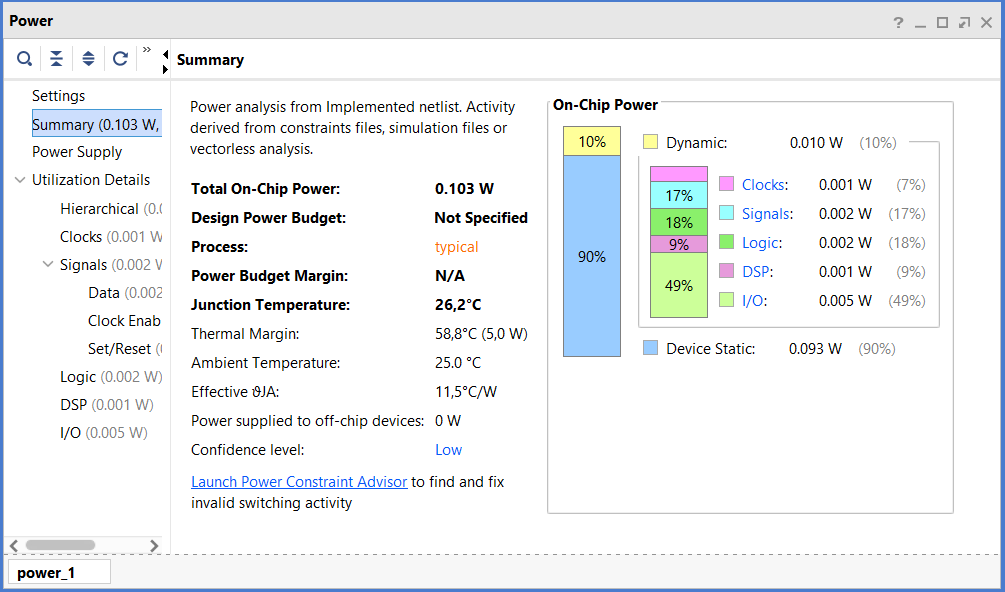
\includegraphics[width=\textwidth]{./images/Vivado/power_report.png}
    \caption{Vivado Power Report after implementation.}
    \label{fig:power_report}
\end{figure}
The power report highlights a total on-chip power consumption of 0.103 W, with 90\% attributed to static power (0.093 W) and 10\% to dynamic power (0.010 W). The dynamic power is distributed among different components: clocks (7\%), signals (17\%), logic (18\%), DSP (9\%), and I/O (49\%), with I/O being the highest consumer of dynamic power. It is important to note that this device will not be used alone but is being connected to I/O pins solely for testing purposes.

The high value of static power over dynamic power is largely to be attributed to the fact that the design is using very little of the available hardware. With reference to the Utilization Report in Chapter \ref{chap:utlization_report}, resources like Slice LUTs and Registers are used only for 2.05\% and 0.32\%, this makes the overall switching activity of the chip very small.

\section{Conclusions}


\chapter{Final considerations}
The design process adopted in this work demonstrates an efficient approach to implementing the CORDIC algorithm. The iterative methodology ensures high accuracy while maintaining low resource utilization, as confirmed by the Vivado synthesis and power analysis reports. 

It is important to note that while the implemented circuit is tailored for the constraints of the Zybo board, the modularity of the design makes it adaptable to other hardware platforms. The testing and verification phase, which included testbenches and graphical analysis, validated the functionality and robustness of the system across a wide range of input conditions.

\nocite{*}
\printbibliography

\end{document}
% -----------------------------------------------------------------
